%-------------------------------------------------------------------------------------------------------
%	TO DO:		- fertig werden
%				- xxx
%-------------------------------------------------------------------------------------------------------

\documentclass[
	%
	journal,
	%compsoc,
	a4paper,
%	onecolumn,
]{IEEEtran}

%-------------------------------------------------------------------------------------------------------
%	Pakete
%-------------------------------------------------------------------------------------------------------

\usepackage[utf8]{inputenc}
\usepackage[T1]{fontenc}
\usepackage[ngerman]{babel}

%\usepackage[
%	backend=biber,
%	style=ieee,
%]{biblatex}
%\usepackage{csquotes}

\usepackage{graphicx}
\usepackage{caption}
\usepackage{xcolor}
\usepackage{amsmath}		%Formlen einbinden
%\usepackage{booktabs}		%Bessere Tabellen
\usepackage[
	locale=DE,
	detect-all,
	per-mode=fraction,
]{siunitx}%		%Einheiten darstellen

\usepackage{flushend}

\usepackage{hyperref}

%-------------------------------------------------------------------------------------------------------
%	Befehle
%-------------------------------------------------------------------------------------------------------

\graphicspath{{Anhang}}

%\addbibresource{quellen.bib}

\newcommand\MYhyperrefoptions{
	bookmarks=true,
	bookmarksnumbered=true,
	pdfpagemode={UseOutlines},
	plainpages=false,
	pdfpagelabels=true,
	colorlinks=true,
	linkcolor={green},
	citecolor={green},
	urlcolor={green},
	pdftitle={Spice Aufgabe},%<!CHANGE!
	pdfsubject={LEN},%<!CHANGE!
	pdfauthor={Jan Hoegen},%<!CHANGE!
	%pdfkeywords={}%<^!CHANGE!
}

%\hypersetup{%
%	colorlinks=true,
%	linkcolor=blue,	
%}

\markboth{Karlsruher Institut für Technologie. Institut für Biomedizinische Technik.}{Hoegen: Spice-Aufgabe der Vorlesung Lineare elektische Netze WS 2020/2021}

\newcommand{\aufgabe}[1]{\emph{Aufgabe #1}}

\newcommand{\bildbreite}{0.95\columnwidth}

%-------------------------------------------------------------------------------------------------------
%	Titel
%-------------------------------------------------------------------------------------------------------

\title{Spice-Aufgabe der Vorlesung Lineare elektische Netze WS 2020/2021}

\author{%
	Jan~Hoegen\\
	Matrikelnummer 2352525\\
	ugyto@student.kit.edu
%	\thanks{Hallo}
	\IEEEcompsocitemizethanks{%
		\IEEEcompsocthanksitem{Jan Hoegen ist eingeschrieben für den Studiengang Elektro- und Informationstechnik am Karlsruher Institut für Technologie. Matrikelnummer: 2352525. E-Mail: ugyto@student.kit.edu}
	}
}

%-------------------------------------------------------------------------------------------------------
%	Beginn
%-------------------------------------------------------------------------------------------------------

\begin{document}

%-------------------------------------------------------------------------------------------------------
%	Abstract
%-------------------------------------------------------------------------------------------------------

\IEEEtitleabstractindextext{%
\begin{abstract}
	In diesem Dokument werden die Lösungen von Jan Hoegen (Matrikel-Nr. 2352525) zur Spice-Aufgabe der Vorlesung \emph{lineare elektrische Netze} präsentiert. Die Vorlesung ist Bestandteil des Studiengangs \emph{Elektro- und Informationstechnik} am Karlsruher Institut für Technologie im Wintersemester 2020. Die eidesstattliche Erklärung findet sich im Anhang \ref{app:eidesstattliche}.\par
	
	Der Seitenstil ist an den IEEE-Standard angelehnt, außerdem wurde auf eine ausführliche Erklärung der verwendeten Größen und Formeln verzichtet. Alle verwendeten Größen, Einheiten und Ausgangsformeln finden sich entweder in der Aufgabenstellung oder im Skript zur Vorlesung \emph{lineare elektrische Netze} von Prof. Dr. rer. nat. O. Dössel.
\end{abstract}}

%-------------------------------------------------------------------------------------------------------
%	Titel & Abstract asugeben
%-------------------------------------------------------------------------------------------------------

\maketitle

\IEEEdisplaynontitleabstractindextext

%\tableofcontents

%-------------------------------------------------------------------------------------------------------
%	Einleitung
%-------------------------------------------------------------------------------------------------------

%\ifCLASSOPTIONcompsoc
%\IEEEraisesectionheading{\section{Einleitung}\label{sec:Einleitung}}
%\else
%\section{Einleitung}
%\label{sec:Einleitung}
%\fi
%
%\IEEEPARstart{T}{his} demo file is intended to serve as a ``starter file''
%for IEEE Computer Society journal papers produced under \LaTeX\ using
%IEEEtran.cls version 1.8b and later.

\hfill 29. Januar 2021

%-------------------------------------------------------------------------------------------------------
%	Inhalt
%-------------------------------------------------------------------------------------------------------

\section{Lösungen zur Aufgabe 1}
Nachfolgend wird die Impedanz und Admittanz eines Schwingkreises aus der \aufgabe{1} betrachtet.

	\subsection*{Aufgabe 1a}
	Die Gesamtimpedanz \(\underline{Z}(\omega)\) berechnet sich mit:
	\begin{subequations}	
	\begin{align}
		\underline{Z}(\omega)&=R_{Last}+(R+\underline{Z_L})\left\vert\right\vert \underline{Z_C}\\
		\intertext{Durch einsetzen der Impedanzen und Umformung ergibt sich:}
		\underline{Z}(\omega)&=R_{Last}+\cfrac{\cfrac{R}{j\omega C}+\cfrac{j\omega L}{j\omega C}}{R+j\omega L+\cfrac{1}{j\omega C}}\\
		\intertext{Um die Doppelbrüche zu entfernen wird nun mit \(\frac{j\omega C}{j\omega C}\) multipliziert. Anschließend kann mit \(\frac{-j\omega CR-\omega^2 CL +1}{-j\omega CR-\omega^2 CL +1}\) komplex konjugiert erweitert werden.}
		\underline{Z}(\omega)&=R_{Last}+\frac{R+j\omega L}{j\omega CR-\omega^2 CL +1}\\
		\begin{split}
			\underline{Z}(\omega)&=R_{Last}+\\[1ex]		
			&\frac{(R+j\omega L)\cdot(-j\omega CR-\omega^2 CL+1)}{(j\omega CR-\omega^2 CL +1)\cdot(j\omega CR+\omega^2 CL +1)}
		\end{split}
		\intertext{Indem die dritte binomische Formel auf den Nenner angewandt wird und weitere Umformungsschritte durchgeführt werden ergibt sich:}
		\begin{split}		
			\underline{Z}(\omega)&=R_{Last}+\frac{R}{\left(1-\omega^{2} L C\right)^{2}+\omega^{2} R^{2} C^{2}}\\[1ex]
			&-j \frac{\omega^{3} L^{2} C+\omega\left(R^{2} C-L\right)}{\left(1-\omega^{2} L C\right)^{2}+\omega^{2} R^{2} C^{2}}\label{eq:Zett}
		\end{split}
	\end{align}
	\end{subequations}
	
	Nach Real- und Imaginärteil getrennt lässt sich somit ablesen:
	\begin{align}
		Re\{\underline{Z}(\omega)\}&=R_{Last}+\frac{R}{\left(1-\omega^{2} L C\right)^{2}+\omega^{2} R^{2} C^{2}\label{eq:ZettReal}}\\[1ex]
		Im\{\underline{Z}(\omega)\}&=-\frac{\omega^{3} L^{2} C+\omega\left(R^{2} C-L\right)}{\left(1-\omega^{2} L C\right)^{2}+\omega^{2} R^{2} C^{2}}
	\end{align}		
	
	\subsection*{Aufgabe 1b}
	Wenn Strom und Spannung in einem Schaltkreis in Phase verlaufen, ist der Imaginärteil beider Größen jeweils \(0\). Darum muss in der \aufgabe{1b} gelten \(Im\{Z(\omega)\}=0\). Da der Nenner nicht Null werden darf, kann dieser vernachlässigt werden.
	\begin{subequations}
	\begin{align}
		Im\{\underline{Z}(\omega)\}=0\Longleftrightarrow&0=-\frac{\omega^{3} L^{2} C+\omega\left(R^{2} C-L\right)}{\left(1-\omega^{2} L C\right)^{2}+\omega^{2} R^{2} C^{2}}\\[1ex]
		&0 =-\omega\cdot(\omega^2 L^2 C + (R^2 C -L))\\
		\intertext{Indem \(\omega\) ausgeklammert wird, lässt sich bereits die erste Lösung ablesen, sie liegt bei \(\omega_{01}=0\). Somit ist \(f_{01}=\frac{1}{2\pi}\cdot\omega_{01}=\SI{0}{\hertz}\). Die zweite Lösung lässt sich durch Nullsetzen des eingeklammerten Terms berechnen:}
		&0=\omega^2_{02} L^2 C+R^2 C -L\\[1ex]
		&\omega_{02}=\sqrt{\frac{-R^2C+L}{L^2C}}\label{eq:omeaga}
	\end{align}		
	\end{subequations}
	
	Dieser Term wird nun in \(f_{02}\) eingesetzt, damit lautet das Ergebnis:
	\begin{equation}
		f_{02}=\frac{1}{2\pi}\cdot\omega_{02}=\frac{1}{2\pi}\cdot\sqrt{\frac{-R^2C+L}{L^2C}}=\SI{23,87}{\hertz}
	\end{equation}
	
	\subsection*{Aufgabe 1c}
	Für die Frequenzwerte \(f_{01}\) und \(f_{02}\) muss lediglich der Realteil der Impedanz betrachtet werden, dies geht aus der vorherigen Aufgabenstellung hervor. Um die Impedanz der Frequenz \(f_{01}\) zu bestimmen gilt \(\omega=0\) in \eqref{eq:ZettReal}, \(f_{02}\) wird durch \eqref{eq:omeaga} in \eqref{eq:ZettReal} berechnet.. Für \(Z(f=\SI{60}{\hertz})\) jedoch wird \eqref{eq:omeaga} und die Gleichung \eqref{eq:Zett} verwendet.
	\begin{align}
		&Z(f_{01})=Z(0)=R_{Last}+R=\SI{120}{\ohm}\\[1ex]
		\begin{split}
			&Z(f_{02})=Z(\omega_{02})=R_{Last}\\
			&+\frac{R}{\left(1-{\frac{-R^2C+L}{L^2C}} LC\right)^2+{\frac{-R^2C+L}{L^2C}} R^2 C^2}=\SI{200}{\ohm}\\
		\end{split}\\[1ex]
		\begin{split}		
			&\underline{Z}(f=\SI{60}{\hertz})=\underline{Z}(\omega=2\pi\cdot\SI{60}{\hertz})\\
			&=\SI{65,99}{\ohm}-j\SI{93,76}{\ohm}
		\end{split}
 		\end{align}
	
	\subsection*{Aufgabe 1d}
	Die Abbildung \ref{fig:1d:Schaltplan} zeigt den Schaltplan zur \aufgabe{1d}. Abbildungen \ref{fig:1d:Impedanz} und \ref{fig:1d:Admittanz} zeigen die Impedanz beziehungsweise Admittanz auf der komplexen Widerstandsebene.
	\begin{figure}
		\centering
		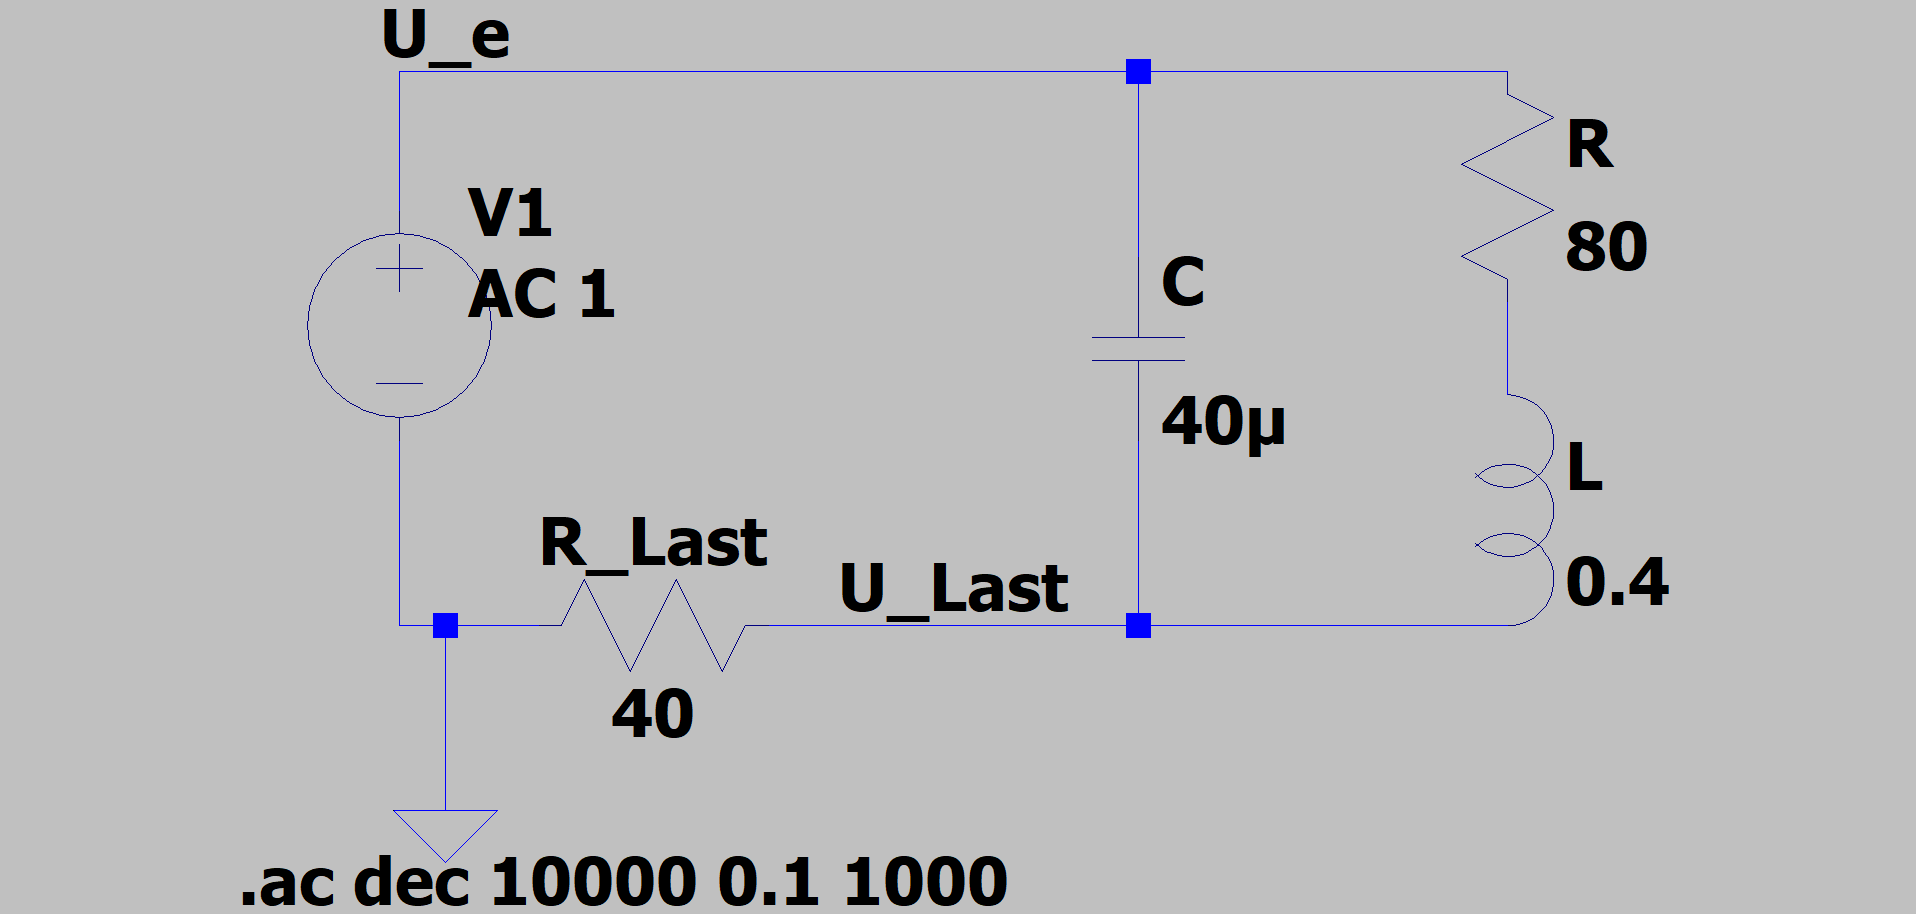
\includegraphics[width=\bildbreite]{Schaltplan.png}
		\caption{Schaltplan zur Aufgabe 1d}			
		\label{fig:1d:Schaltplan}
	\end{figure}
	
	\begin{figure}
		\centering
		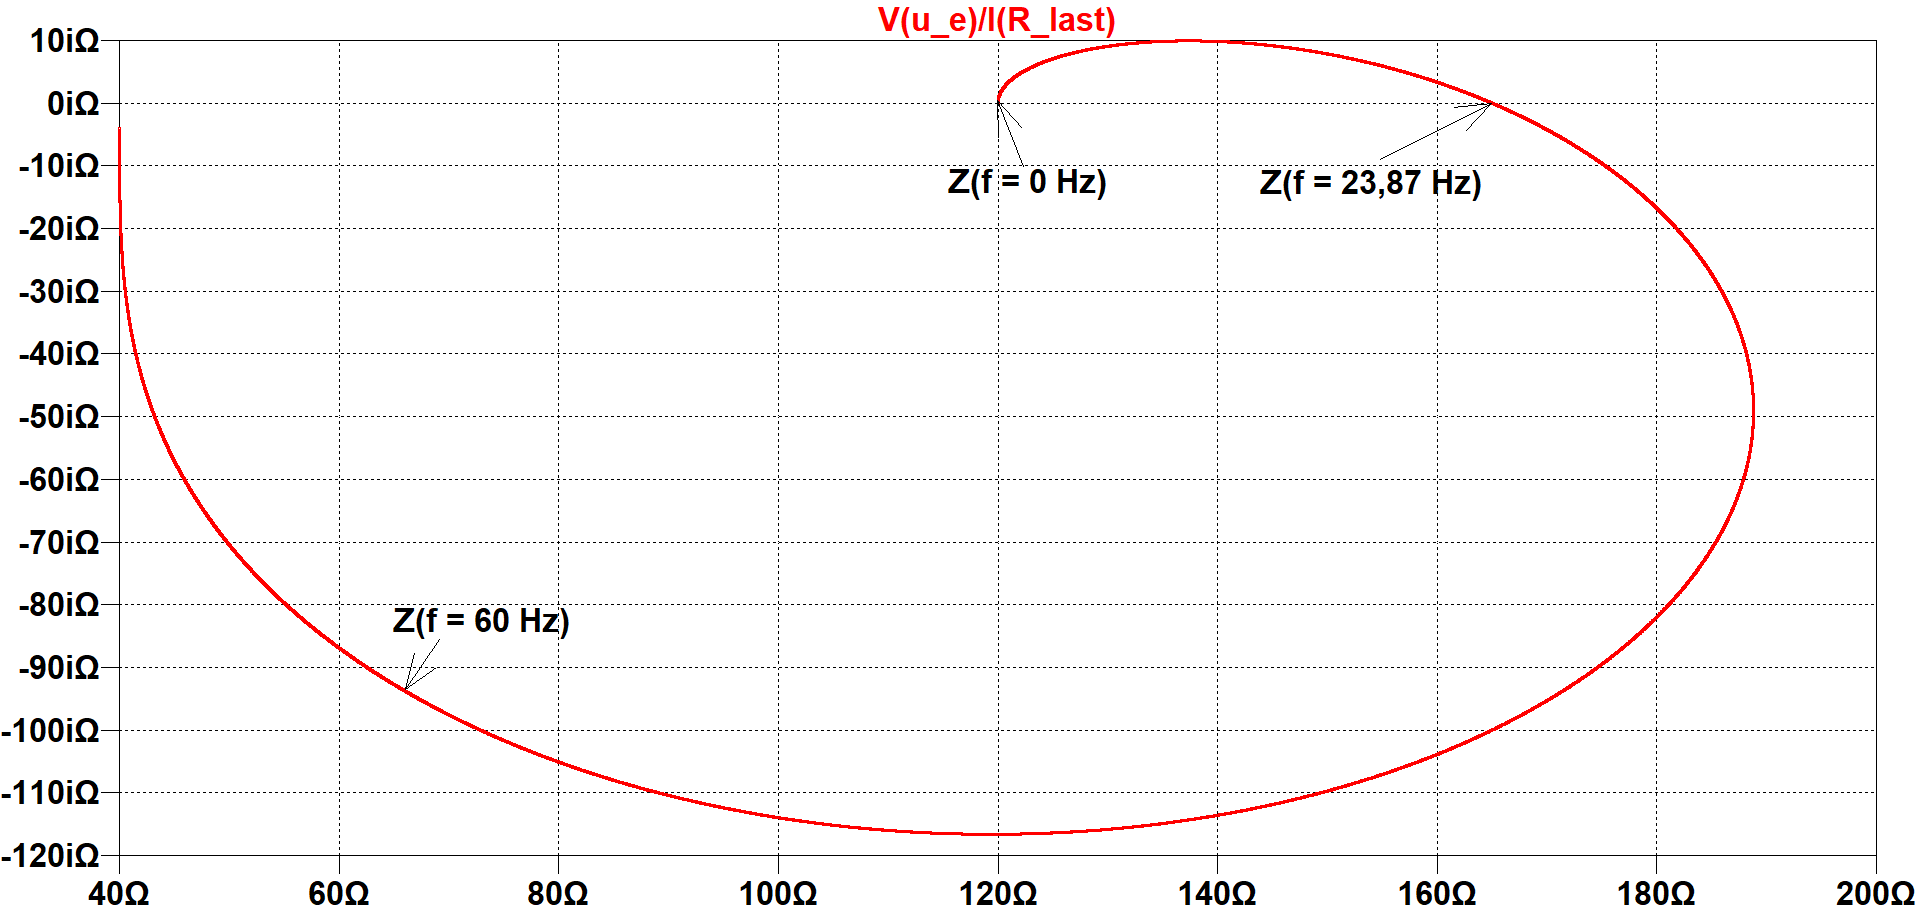
\includegraphics[width=\bildbreite]{Impedanz.png}
		\caption{Impedanz der Aufgabe 1e}
		\label{fig:1d:Impedanz}
		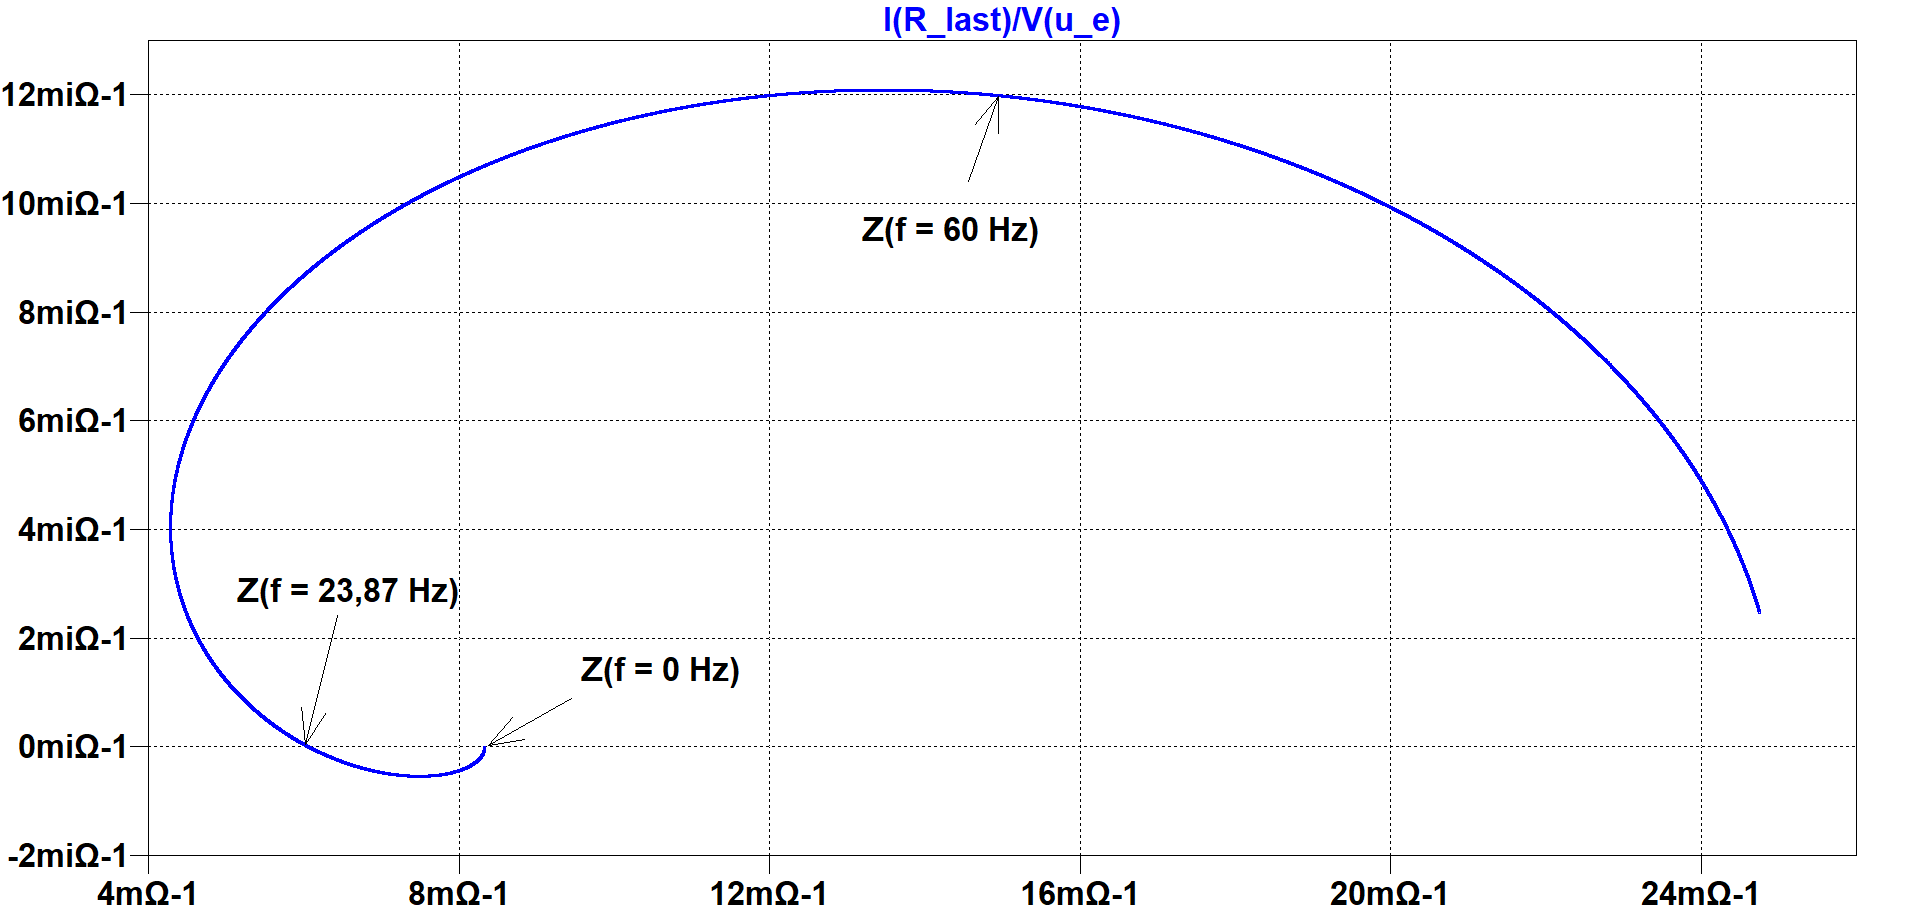
\includegraphics[width=\bildbreite]{Admittanz.png}
		\caption{Admittanz der Aufgabe 1e}
		\label{fig:1d:Admittanz}
	\end{figure}
	
\section{Lösungen zur Aufgabe 2}
In diesem Abschnitt wird ein invertierender Verstärker aus der \aufgabe{2} betrachtet.

\begin{figure}
	\centering
	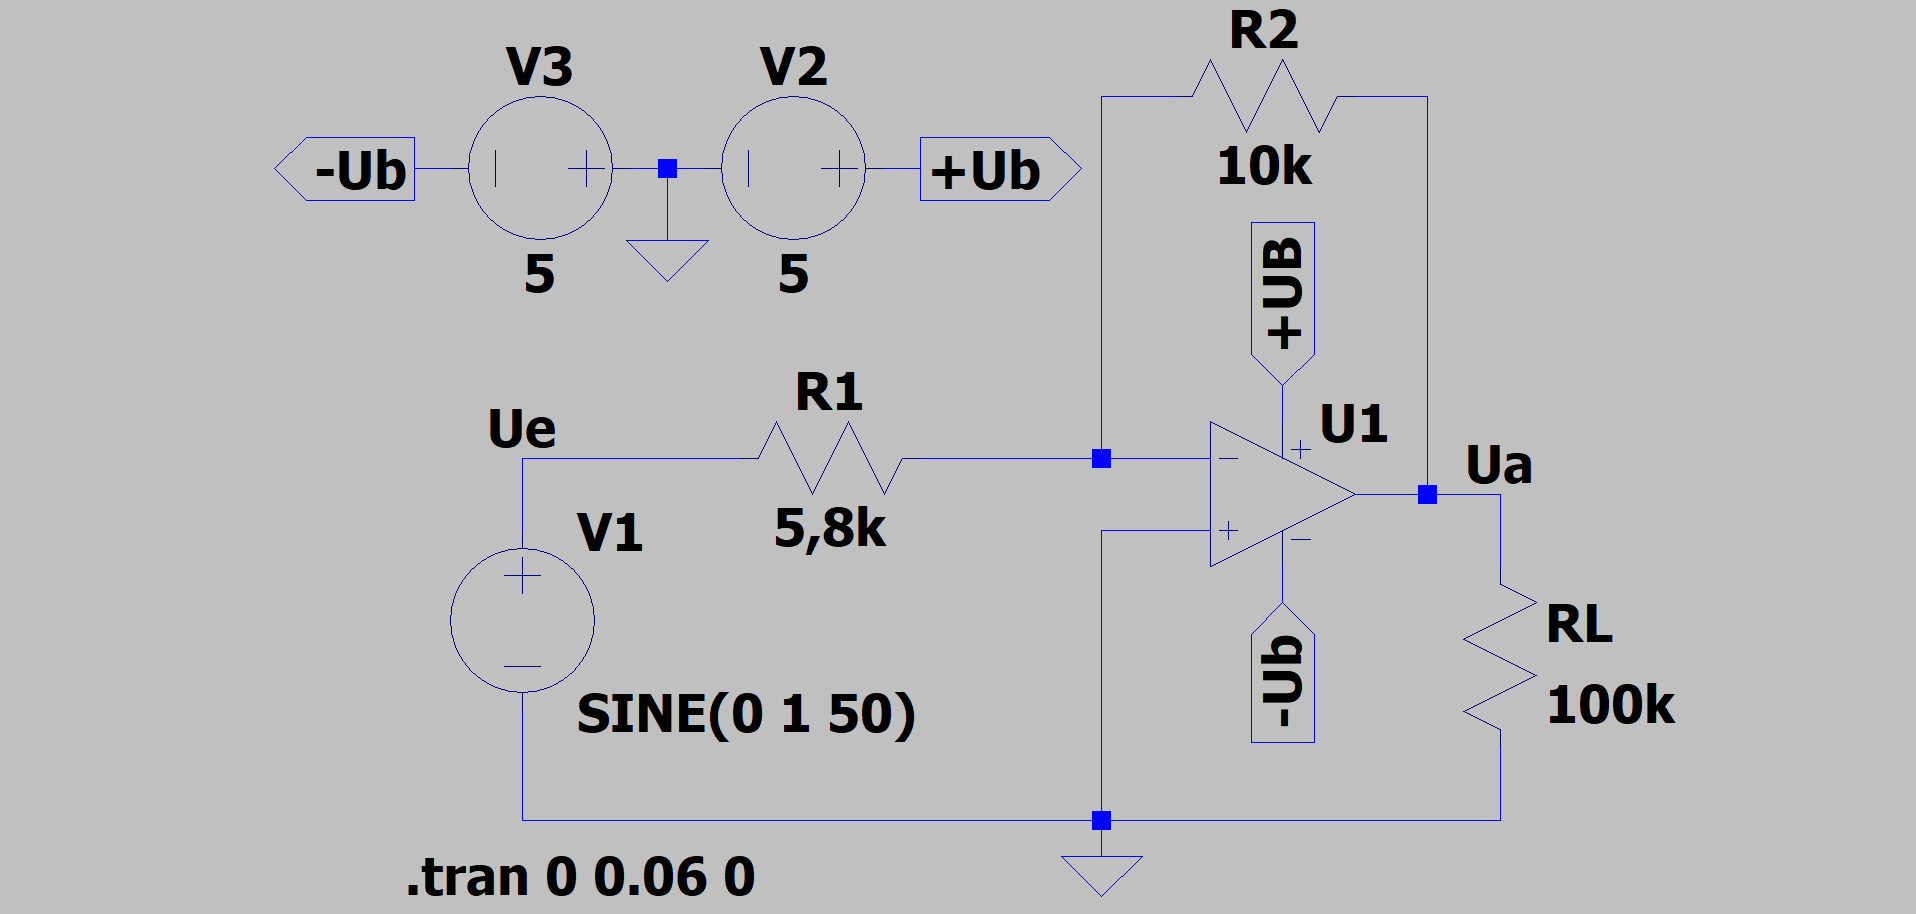
\includegraphics[width=\bildbreite]{2cSchaltplan}
	\caption{Schaltplan zur Aufgabe 2c}
	\label{fig:2c:Schaltplan}
\end{figure}

	\subsection*{Aufgabe 2a}
	Die Maschengleichungen der \aufgabe{2} berechnen sich durch:
	
	\begin{align}
		M1:\quad &0=-U_e + R_1\cdot I_1 \Longleftrightarrow U_e=R_1\cdot I_1\label{eq:2a:Ue}\\
		M2:\quad &0=R_2\cdot I_1+U_a \Longleftrightarrow U_a=-R_2\cdot I_1\label{eq:2a:Ua}
	\end{align}
	
	Das Verhältnis \(\frac{U_a}{U_e}\) vereinfacht sich unter Zuhilfenahme von \eqref{eq:2a:Ue} und \eqref{eq:2a:Ua} zu:
	\begin{equation}
		\frac{U_a}{U_e}=\frac{R_2\cdot I_1}{-R_1\cdot I_1}=-\frac{R_2}{R_1}\label{eq:2a:verhaltnis}
	\end{equation}		
	
	\subsection*{Aufgabe 2b}
	Eine Phasenverschiebung um \(\pi\) wird durch das negative Vorzeichen der Übertragungsfunktion \eqref{eq:2a:verhaltnis} erreicht. Der Verstärkungsfaktor \(2\) wird erreicht, wenn \(R_1\) mit
	
	\begin{equation}
	\begin{split}
		U_a=-2U_e &\Longleftrightarrow -2=\frac{U_a}{U_e}\Longleftrightarrow -2=-\frac{R_2}{R_1}\\[1ex]
		&\Longleftrightarrow R_1=\frac{R_2}{2}=\frac{\SI{10}{\kilo\ohm}}{2}=\SI{5}{\kilo\ohm}
	\end{split}
	\end{equation}
	dimensioniert wird.
	
	\subsection*{Aufgabe 2c}
	Die Abbildungen \ref{fig:2c:Schaltplan} und \ref{fig:2c:Kurven} zeigen den Schaltplan sowie den zeitlichen Verlauf von \(U_a\) beziehungsweise \(U_b\) der \aufgabe{2c}.
	
	\subsection*{Aufgabe 2d}
	Die zu erwartende Ausgangsspannung beträgt 
	\begin{equation}
	\begin{split}
		U_{a,erwartet}&=-\frac{R_2}{R_1}\cdot U_e= -\frac{\SI{10}{\kilo\ohm}}{\SI{5.8}{\milli\ohm}}\cdot \SI{1}{\volt}\\
		&=-\SI{18.97}{\mega\volt}
	\end{split}
	\end{equation}		
	 
	 Der Operationsverstärker jedoch besitzt eine Versorgungsspannung von \SI{5}{\volt}. Da gilt \(U_b\le U_{a,erwartet}\) kann die Ausgangsspannung in dieser Schaltung keine Werte größer als \(U_b\) annehmen. Dies ist auch in Abbildung \ref{fig:2d:Kurven} zu erkennen. Aufgrund der Tatsache, dass weiterhin
	 \(U_b\ll U_{a,erwartet}\) 
gilt, erreicht \(U_a\) bereits bei sehr kleinen Werten für \(U_b\) seine Amplitude. Es entsteht eine Rechteckspannung.

	
	\begin{figure}[t]
		\centering
		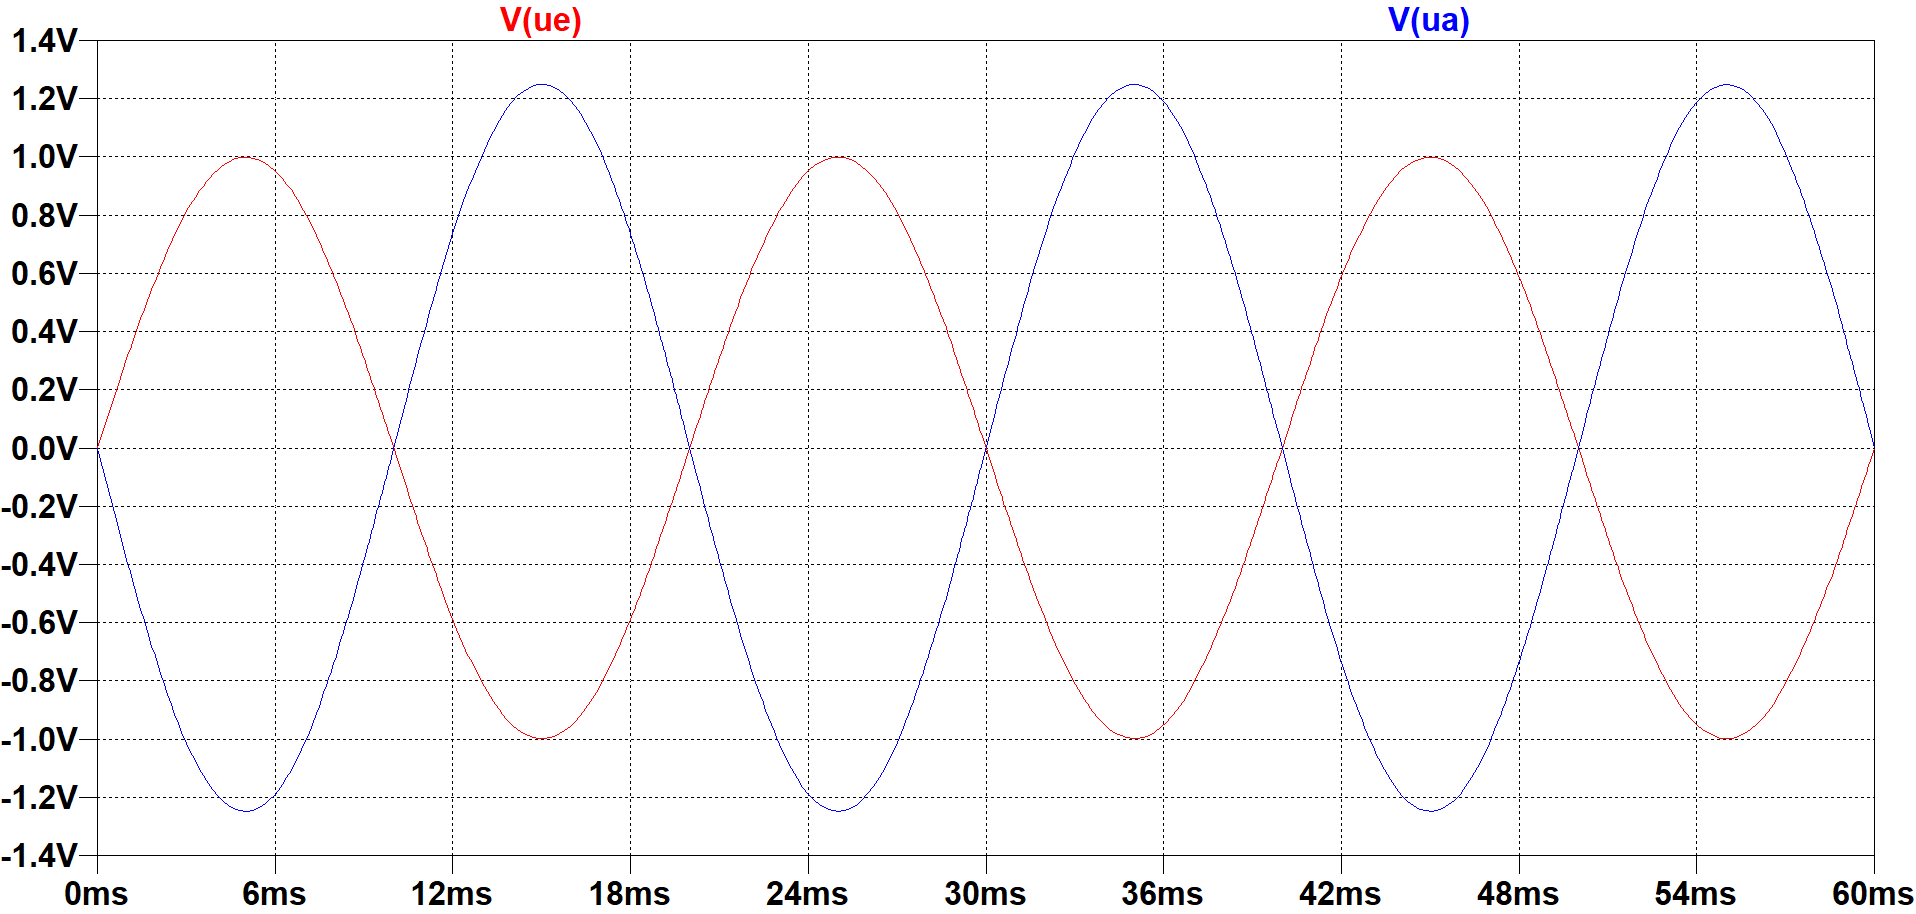
\includegraphics[width=\bildbreite]{2cKurven.png}
		\caption{zeitlicher Verlauf der Spannungen \(U_a\) und \(U_b\)}
		\label{fig:2c:Kurven}
		
		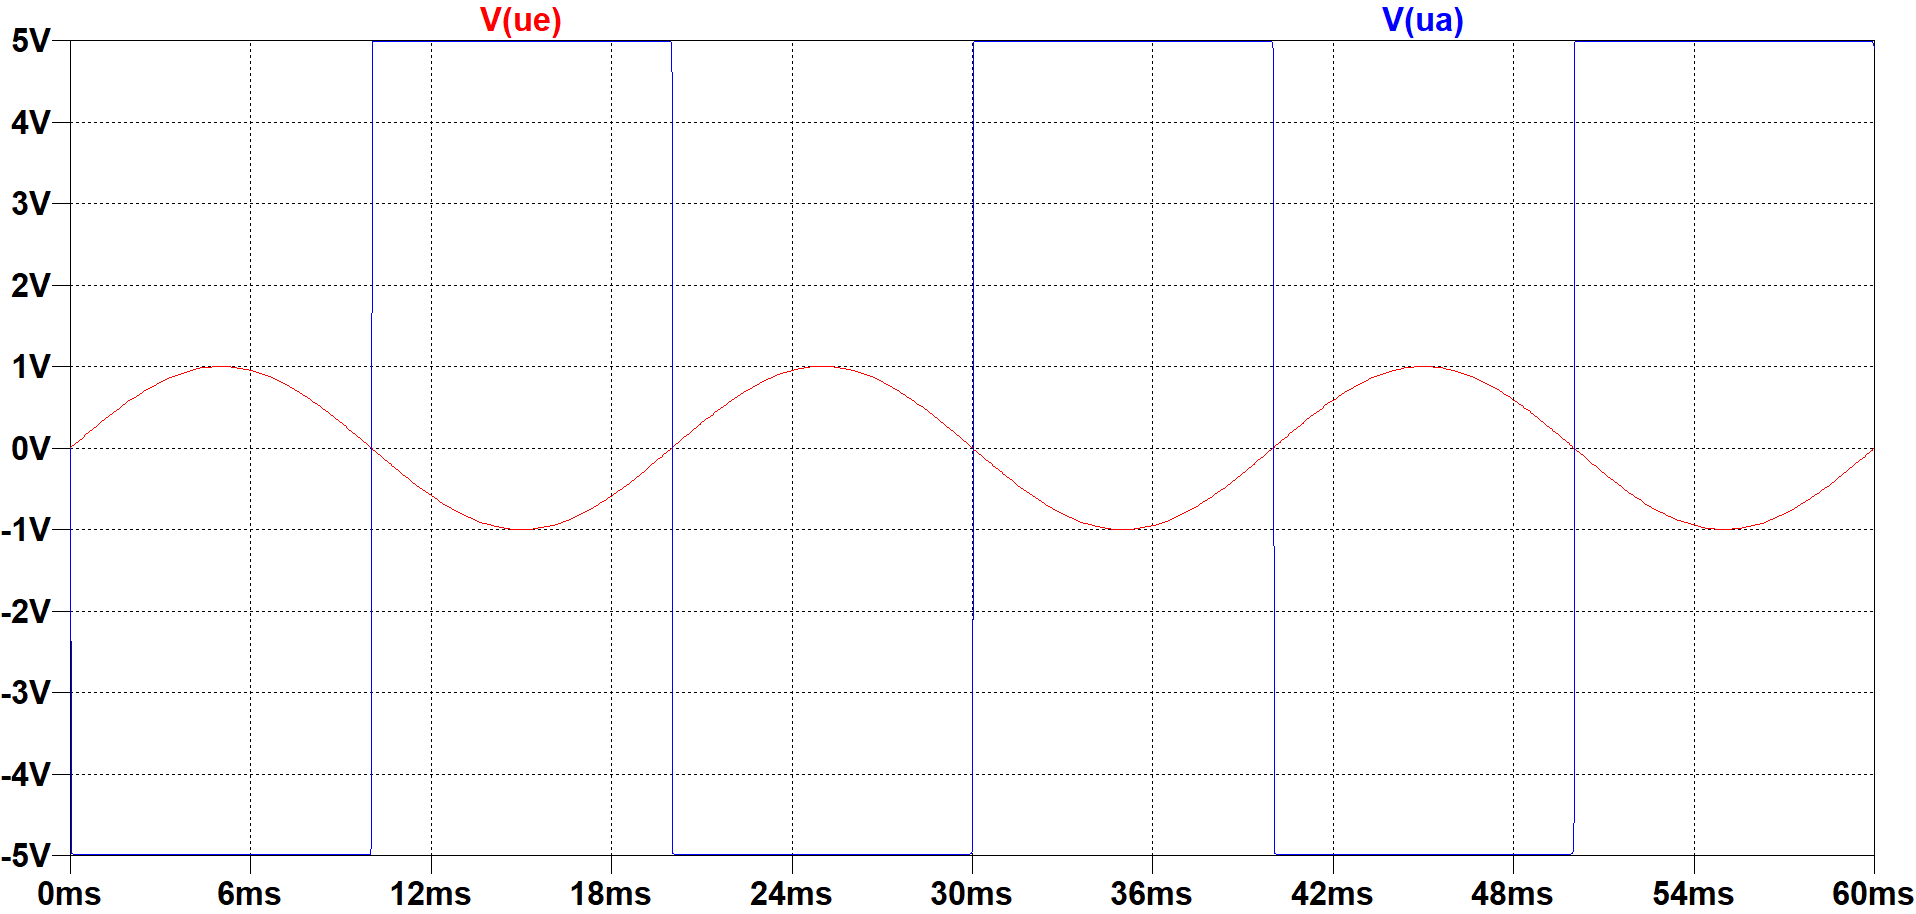
\includegraphics[width=\bildbreite]{2dKurven.png}
		\caption{zeitlicher Verlauf bei \(R_1=\SI{5.8}{\milli\ohm}\)}
		\label{fig:2d:Kurven}
	\end{figure}

%\cite{greenpeace}

%\section{Fazit}
%Lorem ipsum

%-------------------------------------------------------------------------------------------------------
%	Anhang
%-------------------------------------------------------------------------------------------------------

%\appendix
%Anhang

%\appendix[Eidesstattliche Erklärung]

\appendices

%-------------------------------------------------------------------------------------------------------
%	Eidesstattliche Erklärung
%-------------------------------------------------------------------------------------------------------


\section{Eidesstattliche Erklärung}
\label{app:eidesstattliche}
Hiermit erkläre ich an Eides statt, dass ich die vorliegende Arbeit selbstständig und
ohne unzulässige fremde Hilfsmittel angefertigt habe. Wörtlich oder inhaltlich übernommene Stellen sind als solche kenntlich gemacht und die verwendeten Literaturquellen im Literaturverzeichnis vollständig angegeben. Die „Regeln zur Sicherung guter wissenschaftlicher Praxis im Karlsruher Institut für Technologie (KIT)“ in ihrer gültigen Form wurden beachtet.

\vspace{3em}
%\center{
\noindent
\rule{0.9\linewidth}{0.5pt}\\
Ort, Datum \qquad\qquad Jan Hoegen
%}

%-------------------------------------------------------------------------------------------------------
%	Literaturverzeichnis
%-------------------------------------------------------------------------------------------------------

%\printbibliography

%-------------------------------------------------------------------------------------------------------
%	Ende
%-------------------------------------------------------------------------------------------------------

\end{document}